\pagestyle{empty}

% Title page
\sffamily
\begin{center}
	\includegraphics{logo-muni}
\end{center}
\begin{center}
	\huge Přírodovědecká fakulta
\end{center}
\hrule
\vfill

\begin{flushleft}
\huge\noindent
\textbf{\thetitle}
\end{flushleft}
\bigskip

\large\noindent
Diplomová práce
\bigskip

\Large\noindent
\theauthor
\vfill

\Large\noindent
Vedoucí práce: doc. Mgr. Pavel Dvořák, PhD.
\bigskip

\Large\noindent
Ústav fyziky a~technologií plazmatu
\hfill
Brno, 2024

\normalsize
\rmfamily
\cleardoublepage

% Bibliographic entry
\def\bibentryspacing{2}
\chapter*{Bibliografický záznam}
\thispagestyle{empty}
\bgroup
\renewcommand{\arraystretch}{\bibentryspacing}
\begin{tabularx}{\textwidth}{l X}
	\textbf{Autor}            & \theauthor\par
	                            Přírodovědecká fakulta,
	                            Masarykova univerzita\par
	                            Ústav fyziky a~technologií plazmatu \\
	\textbf{Název práce}      & \thetitle \\
	\textbf{Studijní program} & Fyzika \\
	\textbf{Studijní obor}    & Fyzika plazmatu a~nanotechnologií \\
	\textbf{Vedoucí práce}    & doc. Mgr. Pavel Dvořák, PhD. \\
	\textbf{Akademický rok}   & 2023/2024 \\
	\textbf{Počet stran}      & \pageref*{lastpage} \\
	\textbf{Klíčová slova}    & plasma, pikosekundový laser,
	                            nelineární optika,
	                            laserem indukovaná fluorescence,
	                            \EFISH{}\\
\end{tabularx}
\egroup
\cleardoublepage
\chapter*{Bibliographic Entry}
\thispagestyle{empty}
\bgroup
\renewcommand{\arraystretch}{\bibentryspacing}
\begin{tabularx}{\textwidth}{l X}
	\textbf{Author}           & \theauthor\par
	                            Faculty of Science, Masaryk University\par
	                            Department of Plasma Physics and Technology \\
	\textbf{Title of Thesis}  & Plasma diagnostics by means of a picosecond laser \\
	\textbf{Degree Programme} & Physics \\
	\textbf{Field of Study}   & Plasma Physics and Nanotechnology \\
	\textbf{Supervisor}       & doc. Mgr. Pavel Dvořák, PhD. \\
	\textbf{Academic year}    & 2023/2024 \\
	\textbf{Number of Pages}  & \pageref*{lastpage} \\
	\textbf{Keywords}         & plasma, picosecond laser,
	                            nonlinear optics,
	                            laser-induced fluorescence,
	                            \EFISH{} \\
\end{tabularx}
\egroup

% Abstract
\chapter*{Abstrakt}
Tato práce se zabývá metodami využití rychlých pulzních laserů
při diagnostice plazmatu a~jiných průhledných prostředí.
Z~naskýtajících se možností byly zvoleny dvě metody.
Laserem indukovaná fluorescence (LIF)
je zde aplikována na~stanovení absolutní
hustoty selenových atomů ve vodíkovém difuzním plameni.
Méně obvyklým krokem je práce v~částečně saturovaném stavu,
který ztěžuje vyhodnocení a~vyžaduje, aby kromě intenzity fluorescenčního
záření a~doby života byl změřen i~takzvaný saturační parametr.
Metoda je kalibrována Rayleighovým rozptylem.
Výsledkem je prostorově rozlišená hustota atomů selenu v~plameni.
Metoda \EFISH{} je použita ke studiu elektrického pole uvnitř atmosférického
Townsendova výboje v~dusíku.
Po kalibraci v~známém elektrickém poli je získán časový vývoj
elektrického pole v~různých místech výbojového prostoru.
\vfill
{\let\clearpage\relax\chapter*{Abstract}}
\thispagestyle{empty}
This thesis deals with methods using short pulse lasers
in plasma and other transparent media diagnostics.
Two applicable methods were studied.
Laser-induced fluorescence is applied for the determination
of absolute number density of selenium atoms in a hydrogen
diffusion flame.
A less common aspect is operation in partially saturated mode,
which poses additional challenges in evaluation
and requires that the so-called saturation parameter be measured
in addition to fluorescence intensity and lifetime.
Rayleigh scattering is used to calibrate the method.
In the end, spatially resolved concentration of selenium atoms is obtained.
\EFISH{} is used to study the electric field in an atmospheric pressure
Townsend discharge in nitrogen.
After calibration in a known electric field, space- and time-resolved
electric field in the discharge area is calculated.

% Assignment
\cleardoublepage
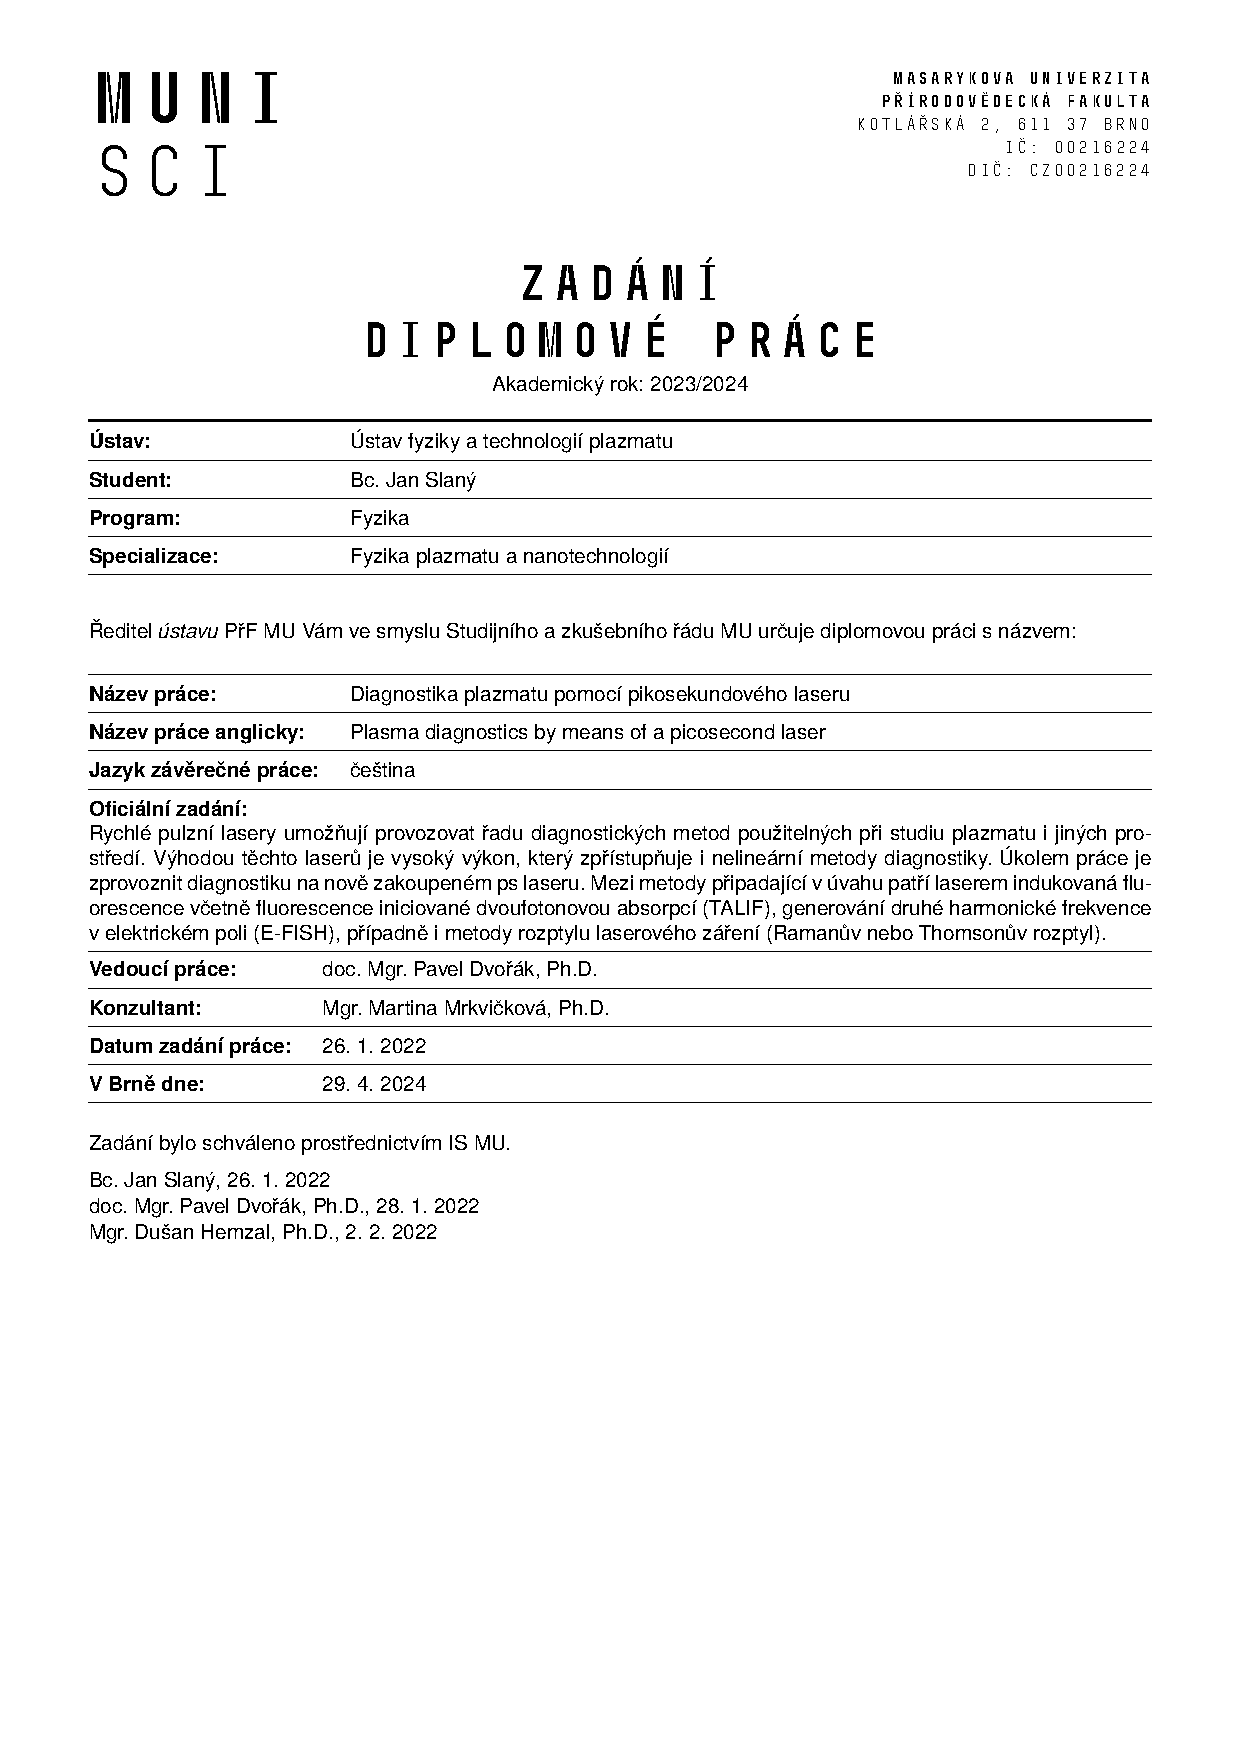
\includepdf[pages={1}]{../zadani.pdf}

% Acknowledgment
\chapter*{Poděkování}
Rád bych tímto poděkoval všem lidem, kteří podporovali mé úsilí
a~bez nichž by tato práce nemohla vzniknout.
Zejména děkuji doc.~Mgr.~Pavlu Dvořákovi, Ph.D.,
a~Mgr.~Martině Mrkvičkové, Ph.D.,
za odborné vedení a~cenné předané zkušenosti.

% TODO: Doplnit korektora
Srdečně děkuji své rodině a~přátelům za oporu, kterou mi byli;
mezi nimi především slečně Ing.~Kláře Welterové za nesmírnou trpělivost.
\vfill

% May be on the same page with acknowledgment
{\let\clearpage\relax\chapter*{Prohlášení}}
\thispagestyle{empty}
Prohlašuji, že jsem svou diplomovou práci vypracoval samostatně
pod vedením vedoucího práce s~využitím informačních zdrojů,
které jsou v~práci citovány.
\bigskip

\noindent
V Brně dne 6.~května~2024
\hfill
\parbox{6cm}{
	\centering
	\vspace{1.5cm}
	\rule{6cm}{0.1pt}\par
	Jan Slaný
}
